\documentclass[]{article}

\usepackage{amsmath}            % align env for aligned equations
\usepackage{enumitem}           % needed for leftmargin ident of the description env
\usepackage{bm}                 % uniform bold with \bm
\usepackage{txfonts}            % conditional independence symbol
\usepackage[linesnumbered,ruled,vlined]{algorithm2e} % algorithm; needs to be laoded before cleverref
\usepackage{cleveref}           % corss-referencing

\usepackage{graphicx}           % figures
\graphicspath{ {fig/} }
\usepackage{epstopdf}

\include{nonpaperheader}
\usepackage{mlmacros}
\usepackage{graphicx}
% \usepackage[draft]{graphicx}
\graphicspath{ {fig/} }
 \usepackage[export]{adjustbox}
 
\usepackage{todonotes}
\usepackage[inline]{enumitem}
\usepackage{bm}

\usepackage{sty/msoelch/mlmacros}
\usepackage{amsmath}
\usepackage{mathtools}
\usepackage{calc}
\usepackage{fontawesome}
\usepackage{hyperref}

%\usepackage[osf,sc]{mathpazo} % Palatino as the main font
%\linespread{1.05}\selectfont % Palatino needs some extra spacing, here 5% extra
% \usepackage[euler-digits]{eulervm} % nicer math font

% \usepackage{floatrow}
\usepackage[skip=5pt]{caption}
\usepackage{subcaption}

\usepackage[noabbrev]{cleveref}

% section spacing
\usepackage{titlesec}

\titlespacing*{\section}
{0pt}{.1\baselineskip}{.1\baselineskip}
  
% Decrease spacing between bib entries
%\setlength{\bibsep}{0pt plus 0.3ex}

\newcommand*{\B}[1]{\ifmmode\bm{#1}\else\textbf{#1}\fi}

\variables{a,b,c,g,t,o,s,v,x,z}
\variables{A,I}

\variables[app]{\alpha}
\variables[mean]{\mu}
\variables[std]{\sigma}
\variables[map]{\nu}
\variables[dparam]{\psi}

% Neil's comment function
\newcommand{\nd}[1]{\textcolor{red}{[ND: #1]}}
\newcommand{\ab}[1]{\textcolor{green}{[AB: #1]}}
\newcommand{\ak}[1]{\textcolor{blue}{[AK: #1]}}

\probdists{p,q}

\DeclarePairedDelimiter{\fences}{(}{)}
\DeclarePairedDelimiter{\norm}{\lVert}{\rVert}

%\DeclareMathOperator{\MLP}{ \mathrm{MLP} \Fences }
\newcommand{\MLP}[1]{ \mathrm{MLP} \fences{#1} }
\newcommand{\LSTM}[1]{ \mathrm{LSTM} \fences{#1} }
\newcommand{\flatten}[1]{ \mathrm{vec} \fences{#1} }

\newcommand{\reg}[1]{ \ensuremath{R} \fences{#1} }

\definecolor{darkgreen}{rgb}{0,.502,0}

\newcommand{\sidecaption}[1]% #1 = label name
{\raisebox{\abovecaptionskip}{\begin{subfigure}[t]{1.6em}
  \caption[singlelinecheck=off]{}% do not center
  \label{#1}
\end{subfigure}}\ignorespaces}

%opening
\title{Attend, Infer, Repeat: Notes}
\author{Adam Kosiorek}


\addbibresource{\string~/Documents/.bib/library.bib}

\begin{document}

\maketitle


\section{Introduction}

    Attend, Infer, Repeat (AIR; \cite{Eslami2016}) is a VAE-type model capable of decomposing a static scene into its constituent parts. This is useful, since it explicitly represent distinct parts of the scene, which provides useful and actionable representations for down-stream processing. An example application are proposal location for object detection algorithms. While not guaranteed to represent objects, parts of the scene represented by separate representations are bound to be statistically significant. The purpose of this document is to explore the model in more detail.
    
\section{Generative Model and Priors}

    Let $\bx$ an image, $n$ a number of statistically interesting separate parts in the image, $\bz = \{\bz^i, \dots, \bz^n \}$ a group of variables, where each variable describes a part of the scene. Let $\p{\bz, n}{}{\theta} = \p{\bz}{n}{\theta}\p{n}{}{\theta}$ be a prior over latent variables describing our assumptions about possible layouts and complexity of the scene and let $\p{\bx}{\bz}{\theta}$ be a \emph{generating} model. The prior and the generating model together form a generative model of the scene, where the prior describes it in terms of latent variables and the generating model uses the latent variables to paint the scene. We can write down the marginal distribution of images as 
    \begin{equation}
        \p{\bx}{}{\theta} = \sum_{n=1}^N \p{n}{}{\theta, N} \int \p{\bz}{n}{\theta} \p{\bx}{\bz}{\theta} \dint \bz.
    \end{equation}
    We take the prior to have the following form:
    \begin{equation}
        \p{n}{}{\theta} = \mathrm{Geom} (n \mid \theta),
    \end{equation}
    \begin{equation}
        \p{\bz}{n}{\theta} = \prod_{i=1}^n \p{\bz^i}{}{\theta} = \prod_{i=1}^n \gauss{\bf{0}, \bf{I}},
    \end{equation}
    which assumes that $\bz^i$ are independent under the prior. The success probability for the geometric distribution is chosen to encourage sparse (as few steps as possible) solutions. In practice, it is annealed over 100k training steps to a very low value on the order of $p = 10^{-e}$,  $e \in [5, 10]$.
    
\section{Inference through an Approximate Posterior}
    
    Since the latent variables $\bz^i$ are independent under the prior, they are exchangeable. It introduces symmetries, which increases the volume of the search space in a combinatorial way. To address this issue, the original work formulates inference as a sequential problem, where latent variables describing a part of a scene depend on previously inferred latent variables. Specifically, it parametrises $n$ as a vector of $n$ ones followed by a zero $\bz^p$. With this representation and a sequential implementation of inference, it is enough to output a single \emph{presence} indicator variable at each processing step. The approximate posterior is given by
    \begin{equation}
        \q{\bz, \bz^p}{\bx}{\phi} = \q{z^{p, n+1} = 0}{\bz^{1:n}, \bx}{\phi} \prod_{i=1}^n \q{\bz^i, z^{p, i} = 1}{\bz^{1:i-1}, \bx}{\phi},
        \label{eq:air_posterior}
    \end{equation}
    with $q_\phi$ implemented as a neural network. To avoid explaining the same object twice, it is vital to capture the dependency $\bz^i, z^{p, i} \mid \bz^{1:i-1}, \bx$, which is implemented as a recurrent neural network $R_\phi$ with hidden state $\bm{h}^i$, where the initial hidden state $\bm{h}^0$ is randomly initialised and learnable, and specifically as
    \begin{equation}
        \bm{\omega}^i, \bm{h}^i = R_\phi (\bx, \bz^{i-1}, \bf{h}^{i-1}).
        \label{eq:air_recurrence}
    \end{equation}
    The variable $\omega^i$ specifies parameters of the probability distribution over $\bz^i$ and $z^{p, i}$ and introduces a conditional independence property, namely $\bz^i \Perp z^{p, i} \mid \omega^i$. We can use this property to factorise the approximate posterior distribution as
    \begin{equation}
          \q{\bz, \bz^p}{\bx}{\phi} = \q{z^{p, n+1} = 0}{\omega^{n+1}}{\phi} \prod_{i=1}^n \q{\bz^i}{\omega^i}{\phi} \q{z^{p, i}}{\omega^i}{\phi}.
          \label{eq:air_factorisation}
    \end{equation}
    Since the hidden state $\bm{h}^i$ is deterministic, it follows a Dirac distribution centred on $\bf{h^i}$ and there is no need to integrate over the it: the integral collapses to a single value. Latent distribution statistics $\bm{\omega}$ are computed iteratively and depend on the previous latent variables. This precludes analytical computation of the KL-divergence, which has to be approximated by sampling.
    
    
\section{Learning by Maximising the ELBO}
    
    AIR is trained by maximising the evidence lower bound $\loss[AIR]$ (ELBO) given by
    \begin{align}
        \loss[AIR]{\phi, \theta} &= \expc{ \log \frac{ \p{\bz, n, \bx}{}{\theta} }{ \q{\bz, n}{\bx}{\phi} } }{}{ \q{}{}{\phi} }\\
        &= \expc{ \log \p{\bx}{\bz}{\theta} }{}{ \q{}{}{\phi} } - \kl{\q{\bz, n}{\bx}{\phi}}{\p{\bz, n}{}{\theta}}.
    \end{align}
    The first term is a probabilistic analog of the reconstruction error, while the second term is a complexity penalty. In this case it encourages minimum-length encoding of every part of the scene as well as decomposing the scene into a minimal number of parts. The KL term can be rewritten  according to the product rule as
    \begin{align}
        &\kl{\q{\bz, n}{\bx}{\phi}}{\p{\bz, n}{}{\theta}} =\\
        &\qquad= \kl{\q{n}{\bx}{\phi}}{\p{n}{}{\theta}} + \expc{ \kl{\q{\bz}{n, \bx}{\phi} }{ \p{\bz}{n}{\theta} } }{}{\q{n}{\bx}{\phi}}.
    \end{align}

\section{Policy Gradient Techniques}
    Policy gradients are used here to backprop through samples from a discrete probability distribution.
    \subsection{Score Function}
        \cite{Williams1992}
        
    \subsection{NVIL}
        \cite{Mnih2014} implemented but doesn't work that well, presumably because of different effective weightings of the continuous and discrete components of the loss. I still have to check with the lower learning rate.
        
    \subsection{Discrete IWAE}
        To be done... Originally introduced by \cite{Burda2015}, but extended to a discrete case by \cite{Tucker2017}.
        
    \subsection{Convex Relaxation}
        To be done... concrete distribution/gumbel \cite{Maddison2016,Jang2016}
        
    \subsection{REBAR}
        This seems terribly complicated \cite{Tucker2017}
        
\section{FIVO for Better Bounds}
    Introduced by \cite{Maddison2017}; ywt says its much better for sequential estimation such as AIR than the usual ELBO.
        
\section{Complex Backgrounds: Behaviour and Extenstions}

    AIR depends on statistical differences between pixels belonging to an object and the ones belonging to the background. Moreover, the way it has been defined, it can reconstruct only objects while neglecting the background completely. It is natural to expect that it simply wouldn't work in the case of non-empty backgrounds. To mitigate this issue, it is necessary to augment the model with a background-explaining component $g$. In a simple case, it could produce a background $\bm{b}$ based on the last hidden state of the controller RNN $R_\phi$, specifically:
    \begin{align}
        \bm{b} &= g_\phi( \bm{(h}^N )\\
        y &= h^{\mathrm{dec}}( \bz, \bm{b})
    \end{align}
    For the case of MNIST, $g$ can be implemented as a simple MLP. For more complicated model, it would have to be a more complicated model based on up-convolutions, but this is also true about the glimpse decoder.
    \todo[inline]{Design an experiment to test this behaviour.}

\section{An Extension to Timeseries}
    AIR displays an inconsistent behaviour depending on initialisation. It is randomly initialised and it tends to converge to different solutions when training is restarted. Only a small subset of the solutions is close to what the user would want, namely explaining one object at a time. This is understandable, since a dataset of single images cannot encode an \emph{consistency} prior, whereby objects would have to be preserved when they move. Extending AIR to sequential data has a potential of solving this issue, since it should be much easier to explain an object by changing its position parameter than to inferring its appearance description from scratch at every time-step. Moreover, it prevents explaining two objects moving separately with a single glimpse, since it would be impossible to preserve them consistently while reconstructing.
    
    An extension to timeseries is not trivial, however. It requires some form of dependency between consecutive timestep. It is important to distinguish temporal and within-timestep dependencies. We dub the latter \emph{sequential} dependencies. In the original work, the only sequential dependencies exist between the hidden states $\bm{h}^i \mid \bm{h}^{i-1}$ and the presence variables $z^{p, i} \mid z^{p, 1:i-1}$, while there is no sequential dependence between appearance and position $\bz^i$. A temporal version of the algorithm requires (or might benefit from) the following:
    \begin{itemize}
        \item between-timestep hidden state dependence \eg $\bm{h}^t \mid \bm{h}^{t-1}$, where this timestep might or might not be the same as the sequential hidden state
        \item temporal dependence on object position
        \item temporal dependence on object appearance
        \item temporal dependence on object presence
        
    \end{itemize}
    
    \subsection{Indian Buffer Process for Object Counts}
        Read and write \citep{Gael2009}.
        
    \section{An Extension to Timeseries: Attend, Propagate, Discover, Repeat (APDR)}
AIR displays an inconsistent behaviour depending on initialisation. It is randomly initialised and it tends to converge to different solutions when training is restarted. Only a small subset of the solutions is close to what the user would want, namely explaining one object at a time. This is understandable, since a dataset of single images cannot encode any \emph{consistency} prior, whereby objects would have to be preserved when they move. Extending AIR to sequential data has a potential of solving this issue, since it should be much easier to explain an object by changing its position parameter than to infer its appearance description from scratch at every time-step. Moreover, it prevents explaining two objects moving separately with a single glimpse, since it would be impossible to preserve them consistently while reconstructing.

An extension to timeseries is not trivial, however. It requires some form of dependency between consecutive time-step. It is important to distinguish temporal and within-time-step dependencies. We dub the latter \emph{sequential} dependencies. In the original work, sequential dependencies exist between the deterministic hidden states and stochastic latent variables, namely $\bm{h}^i \mid \bm{h}^{i-1}, \bz^{i-1}, z^{p, i-1},$ and $\bz^i, z^{p, i} \mid \bm{h}^{i-1}$. A temporal version of the algorithm requires (or might benefit from) the following:
\begin{itemize}
    \item between-time-step hidden state dependence \eg $\bm{h}_t \mid \bm{h}_{t-1}$, where this time-step might or might not be the same as the sequential hidden state
    \item temporal dependence on object position
    \item temporal dependence on object appearance
    \item temporal dependence on object presence
\end{itemize}

\begin{figure}
    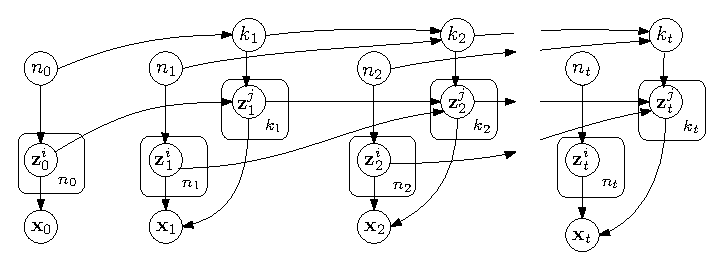
\includegraphics[width=\textwidth]{seq_air}
    \caption{The generative story of sequential AIR.}
    \label{fig:seq_air}
\end{figure}

\begin{figure}
    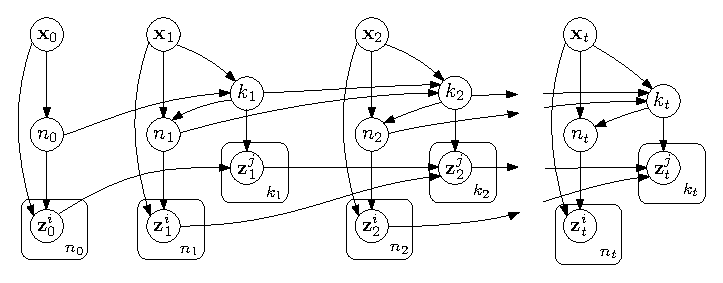
\includegraphics[width=\textwidth]{seq_air_inference}
    \caption{Graphical model for inference in sequential AIR.}
    \label{fig:seq_air_inf}
\end{figure}

\subsection{Sequential Generative Model and Prior}

Let us start by describing the prior generative story. Images are generated by first assuming that, at every time-step, objects are propagated from the previous time-step and some new objects can be introduced (or discovered), where propagation and discovery are handled by different parts of the model. Let $k \in \{0, 1, \dots, K\}$,  the number of objects propagated from the previous time-step and let $n \in \{0, 1, \dots, N - k\}$ the number of objects discovered at the current time-step. The maximum of $K \in \mathcal{N}_+$ objects can be propagated and the model can handle up to $N \in \mathcal{N}_+$ total objects, therefore $K \leq N$. Moreover, at every time-step, the model will generate a set of latent variables, one for each object. If we use superscripts $D$ and $P$ to denote latent variables generated by discovery and propagation models, respectively, then the aggregated latent variable $\bzt = \bzt^P \cup \bzt^D$, where $\bzt^P = \{ \bzt^{P, 1}, \dots, \bzt^{P, \kt} \}$ and $\bzt^D = \{ \bzt^{D, 1}, \dots, \bzt^{D, \nt} \}$. Consequently, if we use $m_t = \kt + \nt$ to denote the total number of objects present at time $t$, then $\bzt = \{ \bzt^1, \dots, \bzt^{m_t} \}$. We note that the structure of the latent variables from the discovery and propagation models is the same, and in its simplest form it consists of $\bzt^i = \{ \bzt^{\mathrm{what}, i}, \bzt^{\mathrm{where}, i}, b_t^i \}$. The components represent appearance, location and presence of an object at the given time-step.

 At the first time-step $t = 1$ there are no objects to propagate, so we sample up to $N$ objects from a discovery prior $\p{n_1, \bz_1^D}{N}$. Starting from the second time-step $t=2$, the model first propagates objects by sampling from a propagation prior $\p{k_2, \bz_2^P}{n_1 + k_1, \bz_1}$, where $\bz_1 = \bz_1^D$. The model also samples $n_2$ new objects from the prior $\p{n_2, \bz_2^D}{N - k_2}$. From now on, that is for $t \geq 2$, we set the aggregated latent variable $\bz_t = \bz_t^P \cup \bz_t^D$. This process continues up to the final time-step $T$. The images are generated by passing the latent variables $\bzTs$ to the generating model $\p{\bxt}{\bzt}{\theta}$ one at a time. Note that $\bzt$ is a set of up to $N$ latent variables, where each latent variable represents a separate object. The generating model acts separately on every latent variable in the set, and the output random variable of the generating model consists of the sum of outputs of the generative model for each latent variable in the set. \Cref{fig:seq_air} shows the graphical model of the generative story. Please note that the prior for the number of new objects stays the same for every time-step and it is analogous to the prior used by AIR, with the exception that the number of maximum objects can differ.

To make it more formal, we will now give all equations governing the generative process. The prior for the discovery model is defined as follows.
\begin{equation}
\begin{aligned}
    \p{n_t, \bzt^D}{N}{\theta} &=\\
    \p{n_t}{N} \p{\bzt}{n_t}{\theta} 
    &= \operatorname{TruncatedGeom} \left( n_t \mid N, \theta \right)
    \prod_{i=1}^{n_t} \gauss{\bf{0}, I},
\end{aligned}
\end{equation}
where $\operatorname{TruncatedGeom} \left( n_t \mid N, \theta \right)$ is a geometric distribution, whose support is truncated to $\{0, 1, \dots, N\}$ and the success probability is given by $\theta$. The propagation model is defined by the following.
\begin{equation}
\begin{aligned}
    \p{k_t, \bzt^P}{m_{t-1}, \bz_{1:t-1}} = \prod_{j=1}^m \p{\bt^{P, j}}{\bz_{1:t-1}^j} \p{\bzt^j}{\bz_{1:t-1}^j} =\\
    \prod_{j=1}^{m_{t-1}} \mathrm{Bernoulli} \left(\bt^{P, j} \mid \psi( \bz_{1:t-1}^j) \right) \gauss{\bzt^j \mid \bm{\mu} (\bz_{1:t-1}^j), \bm{\sigma}^2(\bz_{1:t-1}^j)},
\end{aligned}
\label{eq:prop_prior}
\end{equation}
with $m_t = n_t + k_t$ the total number of objects present at time $t$, $\bz_{1:t-1}^j$ the history of latent variables belonging to object $j$ and $\bz_{1:0}^j = \emptyset$. In the above we reparamterise $k_t$ as a sum of Bernoulli random variables $\bt^{P, j}$, that is $k_t = \sum_{i=1}^m \bt^{P, j}$. Since the probability of propagation $\psi^j$ is different for every object, $k_t$ follows a Poisson-Binomial distribution with $m$ trials. Direct conditioning on the whole history of latent variables is impractical, and therefore we use a learned deterministic RNN $R_\theta^\mathrm{prior}$ to estimate $\psi$, $\mu$ and $\sigma^2$. the RNN shares parameters but maintains a separate hidden state for every object $j$. We can rewrite \Cref{eq:prop_prior} in terms of a simple recurrence as
\begin{equation}
\begin{aligned}
    \p{k_t, \bzt^P}{m_{t-1}, \bz_{1:t-1}} = \p{k_t, \bzt^P}{m_{t-1}, \bm{h}_t^{\mathrm{prior},\ j}} =\\
    \prod_{j=1}^{m_{t-1}} \mathrm{Bernoulli} \left(\bt^{P, j} \mid \psi( \bm{h}_t^{\mathrm{prior},\ j} ) \right) \gauss{\bzt^j \mid \bm{\mu} (\bm{h}_t^{\mathrm{prior},\ j}), \bm{\sigma}^2(\bm{h}_t^{\mathrm{prior},\ j})},
\end{aligned}
\end{equation}
\begin{equation}
    \bm{h}_t^{\mathrm{prior},\ j} = R_\theta^\mathrm{prior} \left( \bz_{t-1}^j, \bm{h}_{t-1}^{\mathrm{prior},\ j} \right).
\end{equation}
Any parameters in the generating model, \eg the parameters of the RNN, can be learnt jointly with the inference model (to be described shortly).
Alternatively, one could use a non-parametric prior for the discrete latent variable $\kTs$, \eg the Indian Buffet Process \citep{Gael2009}, \emph{cf.} \Cref{sec:related_work}. \todo{I should actually use the IBP prior...}

Images are created by decoding the latent variables into small `glimpses' $\widehat{\bg}_t^j \in \RR^{h \times w \times c}$ that are then transformed into partial images $\byt^j \in \RR^{W \times H \times c}$, $w < W$, $h < H$, which match the size of the original image, and they are summed up. More formally, recall that each latent variable $\bzt^j$ contains $\bzt^{j, \mathrm{where}}$ and  $\bzt^{j, \mathrm{what}}$, we have
\begin{equation}
    \widehat{\bg}_t^j = f^{\mathrm{dec}}_\theta \left( \bzt^{\mathrm{what}, j} \right),
\end{equation}
\begin{equation}
    \byt^j = f^{\mathrm{STN}} \left( \widehat{\bg}_t^j, \bzt^{\mathrm{where}, j} \right),
\end{equation}
\begin{equation}
    \bm{\mu}_x = \sum_{j=1}^{m_t} \byt^j,
\end{equation}
\begin{equation}
    \widehat{\bx}_t \sim \gauss{ \bxt \mid \bm{\mu}_x, \bm{\sigma}_x^2},
\end{equation}
with the decoder $f^{\mathrm{dec}}$, spatial transformer $f^{\mathrm{STN}}$ and a fixed per-pixel standard deviation $\bm{\sigma}_x^2$.

All components of the generative model taken together specify a joint probability $\p{\bxTs, \bzTs,\nTs,\kTs}{}{\theta}$ over the sequence of images and the corresponding latent variables. We can expand it as
\begin{equation}
\begin{aligned}
    &\p{\bxTs, \bzTs,\nTs,\kTs}{}{\theta} = \prod_{t=1}^T \p{\bxt, \bzt, \nt, \kt}{\bz_{1:t-1}, n_{1:t-1}, k_{1:t-1}}{\theta}\\
%    
    &\qquad= \prod_{t=1}^T \p{\bxt}{\bzt}{\theta} \p{\bzt, \nt, \kt}{\bz_{1:t-1}, n_{1:t-1}, k_{1:t-1}}{\theta}\\
%    
    &\qquad= \prod_{t=1}^T \underbrace{\p{\bxt}{\bzt}{\theta}}_\mathrm{generation} \quad \underbrace{\p{\bzt^D, \nt}{\bzt^P, \kt}{\theta}}_\mathrm{discovery} \quad \underbrace{\p{\bzt^P, \kt}{\bz_{1:t-1}, n_{1:t-1}, k_{1:t-1}}{\theta}}_\mathrm{propagation}.
\end{aligned}
\end{equation}
In the second line we used the fact that the observation at time $t$ is conditionally independent of latent variables at previous time-steps given the current ones. In the third line we split $\bzt$ as the union of latent variables corresponding to the discovered objects $\bzt^D$ and propagated objects $\bzt^P$. Only the latter depend on the history of latent variables; the former depend only on what is captured in propagation to the current step. The last term can be decomposed as
\begin{equation}
\begin{aligned}
&\p{\bzt^P, \kt}{\bz_{1:t-1}, n_{1:t-1}, k_{1:t-1}}{\theta}\\
%
&\qquad= \int \p{\bzt^P, \kt}{\bz_{t-1}, n_{t-1} + k_{t-1}, \bm{h}_t^P}{\theta} \p{\bm{h}_t^P}{\bm{h}_{t-1}^P, \bz_{t-1}}{\theta} \dint \bm{h}_t^\mathrm{prior}\\
%
&\qquad= \p{\bzt^P, \kt}{\bz_{t-1}, m_{t-1}, \bm{h}_t^\mathrm{prior}}{\theta} \lvert_{\bm{h}_t^\mathrm{prior} = R^\mathrm{prior}_\theta \left( \bm{h}_{t-1}^\mathrm{prior}, \bz_{t-1} \right)},
\end{aligned}
\end{equation}
where we introduce the hidden state $\bm{h}_t^P$ of the RNN used for propagating objects through time. Computation of the state is deterministic and therefore $\p{\bm{h}_t^\mathrm{prior}}{\bm{h}_{t-1}^\mathrm{prior}, \bz_{t-1}}{\theta}$ is a Dirac distribution centred on $\bm{h}_t^P$, which further simplifies computation. In the second line we also used the fact that object propagation depends only on the number of objects present at the previous time-step and it does not matter whether the objects were propagated from previous time-step or newly discovered.

\subsection{Inference}
To infer the latent variables, we have to invert the generative model. To do so, the inference model has to take into account the observations $\bxTs$ and produce sequences of sets of latent variables $\bzTs$. Similar to the generative process, inference uses a two-step approach, whereby it propagates objects from previous time-steps and then tries to discover new objects. Let us start by defining the approximate posterior distribution over all latent variables.
\begin{equation}
\begin{aligned}
    &\q{\bzTs, \nTs, \kTs}{\bxTs}{\phi} \\
%    
    &\qquad= \prod_{t=1}^T  \q{\bzt, \nt, \kt}{\textcolor{red}{\bxts}, \bz_{1:t-1}, n_{1:t-1}, k_{1:t-1}}{\phi}\\
%    
    &\qquad= \prod_{t=1}^T  \q{\bzt, \nt, \kt}{\textcolor{red}{\bxt}, \textcolor{blue}{\bz_{1:t-1}, n_{1:t-1}, k_{1:t-1}}}{\phi}\\
%    
    &\qquad= \prod_{t=1}^T  \q{\bzt, \nt, \kt}{\bxt, \textcolor{blue}{\bz_{t-1}, n_{t-1}, k_{t-1}}, \bm{h}_t^q}{\phi}\lvert_{\bm{h}_t^q = R^q_\phi \left( \bz_{t-1}, \bm{h}_{t-1}^q \right)} \\
%    
    &\qquad= \prod_{t=1}^T  \qd{\bzt^D, \nt}{\bxt, \bzt^P, \kt}{\phi} \qp{\bzt^P, \kt}{\bxt, \bz_{t-1}, \textcolor{red}{k_{t-1} + n_{t-1}}, \bm{h}_t^q}{\phi} \\
%    
    &\qquad= \prod_{t=1}^T  \underbrace{ \qd{\bzt^D, \nt}{\bxt, \bzt^P, \kt}{\phi}}_\mathrm{discovery} \quad \underbrace{\qp{\bzt^P, \kt}{\bxt, \bz_{t-1}, \textcolor{red}{m_{t-1}}, \bm{h}_t^q}{\phi}}_\mathrm{propagation} 
\end{aligned}
\end{equation}
In the second line we use the product rule to rewrite the joint distribution as a temporal chain. In the third line we introduce the assumption that latent variables are conditionally independent of the past observations given the corresponding latent variables. In the fourth line we substituted the dependency on the history of latent variables by introducing a Markovian hidden state $\bm{h}_t^q$. We assume that the hidden state follows a Dirac distribution and therefore the associated integral collapses to a single value. In line five we split the latent variable $\bzt$ into the ones introduced by the discovery and propagation steps, respectively. We also omit the value of the hidden state to reduce clutter. In line six we explicitly condition the propagation step on the number of latent variables in the previous time-step.

We start by describing the propagation model $\qp{}{}{\phi}$. We would like to condition propagation of objects on other propagated objects at the current time-step, and therefore we decompose inference into a sequence of steps.
\begin{equation}
\begin{aligned}
    &\qp{\bzt^P, \kt}{\bxt, \bz_{t-1}, m_{t-1}, \bm{h}_t^q}{\phi}\\
%    
    &\qquad= \prod_{i=1}^{m_{t-1}} \qp{\bzt^{P, i}, \bt^{P, i}}{\bxt, \bz_{t-1}^i, \bm{h}_t^q, \textcolor{red}{\bzt^{P, 1:i-1}}}{\phi}\\
%    
    &\qquad= \prod_{i=1}^{m_{t-1}} \qp{\bzt^{P, i}, \bt^{P, i}}{\bxt, \bz_{t-1}^i, \bm{h}_t^q, \textcolor{blue}{\bm{h}_t^{P, i}}}{\phi} \lvert_{\bm{h}_t^{P, i} = R_\phi^P \left(  \bzt^{P, i-1}, \bt^{P, i-1} \bm{h}_t^{P, i-1} \right)}
\end{aligned}
\end{equation}
$\bzt^{P, 0}$ and $bt^{P, 0}$ start as zeros and  $\bm{h}_t^{P, 0}$ is randomly initialised and learnable. It is worth noting that $m_t = \sum_{i=1}^{m_{t-1}} \bt^{P,i} \leq m_{t-1}$, therefore propagation can forget objects, but it cannot introduce any new ones. At the end of the propagation stage, the hidden state $\bm{h}_t^{P, \kt}$ should contain information about all the propagated objects and can be used to condition the discovery stage.

To handle object discovery, we follow the implementation of AIR, with the difference that we condition on the hidden state of the propagation phase $\bm{h}_t^{P, \kt}$ and that there is a variable maximum number of steps. It defines a sequential inference procedure, where the model attends to and explains different regions of the image, one at a time. The approximate posterior distribution is defined by \Cref{eq:air_posterior,eq:air_recurrence,eq:air_factorisation}.
We redefine it here to account for temporal dependencies and conditioning. The approximate posterior distribution for discovered objects is given by
\begin{equation}
\begin{aligned}
    &\qd{\bzt^D, \nt}{\bxt, \textcolor{red}{\bzt^P}, \kt}{\phi}\\
%    
    &= \qd{\bzt^D, \nt}{\bxt, \textcolor{red}{\bm{h}_t^{P, \kt}}, \kt}{\phi}\\
%    
    &= \qd{\bt^{D, \nt + 1} = 0}{\bxt, \textcolor{blue}{\bzt^{D, 1:\nt}}, \bm{h}_t^{P, \kt}, \kt}{\phi} \prod_{i=1}^{\nt} \qd{\bt^{D, i}, \bzt^{D, i}}{\bxt, \textcolor{blue}{\bzt^{D,1:i-1}}, \bm{h}_t^{P, \kt}, \kt}{\phi}\\
%    
    &= \qd{\bt^{D, \nt + 1} = 0}{\bxt, \textcolor{blue}{\bm{h}_t^{D, \nt}}, \bm{h}_t^{P, \kt}, \kt}{\phi} \prod_{i=1}^{\nt} \qd{\bt^{P, i}, \bzt^{D, i}}{\bxt, \textcolor{blue}{\bm{h}_t^{D, i-1}}, \bm{h}_t^{P, \kt}, \kt}{\phi},\\
%    
%    &\text{where}\\
%    
\end{aligned}
\end{equation}
where
\begin{equation}
\begin{aligned}
    &\qquad \bm{h}_t^{D, i} = R_\phi^D \left( \bzt^{D, i}, \bm{h}_t^{D, i-1} \right),\\
%    
    &\qquad \qd{\bt^{D, i}}{\bxt, \bzt^{D, 1:i}, \bm{h}_t^{P, \kt}, \textcolor{red}{\kt}}{\phi} = 
    \begin{cases}
        \qd{\bt^{D, i}}{\bxt, \bzt^{D, 1:i}, \bm{h}_t^{P, \kt}}, & \text{if}\ i \leq N-\kt \\
        0, & \text{otherwise}
    \end{cases},\\
%    
    &\qquad \qd{\bt^{D, i} \textcolor{blue}{= 0}}{\bxt, \bzt^{D, 1:i}, \bm{h}_t^{P, \kt}, \kt}{\phi} 
    = 1 - \qd{\bt^{D, i}}{\bxt, \bzt^{D, 1:i}, \bm{h}_t^{P, \kt}, \kt}{\phi}.
\end{aligned}
\end{equation}

\subsection{Variational Lower Bound}
Given the specification of the prior distribution and the inference model, we can derive the evidence lower bound (ELBO).
\begin{equation}
\begin{aligned}
    &\loss[APDR]{\phi, \theta} = \expc{ \log \frac{ \p{\bzTs, \nTs, \kTs, \bxTs}{}{\theta} }{ \q{\bzTs, \nts, \kts}{\bxTs}{\phi} } }{}{ \q{}{}{\phi} }\\
    %
    &= \expc{ \log \p{\bxTs}{\bzTs}{\theta} }{}{ \q{}{}{\phi} } \\
%    
    &\qquad \qquad - \kl{\q{\bzTs, \nTs, \kTs}{\bxTs}{\phi}}{\p{\bzTs, \nTs, \kTs}{}{\theta}}.
\end{aligned}
\end{equation}
The KL divergence term cannot be computed analytically due to non-linear temporal dependencies, and we have to resort to a Monte-Carlo approximation. The latter can be rewritten as a sum of per time-step components. 
%\begin{equation}
%\begin{aligned}
%    &\kl{\q{\bzTs, \nTs, \kTs}{\bxTs}{\phi}}{\p{\bzTs, \nTs, \kTs}{}{\theta}}\\
%%    
%    &= \dots\\
%%    
%    &\approx \sum_{t=1}^T \operatorname{KL}_t(\cdot)
%\end{aligned}
%\end{equation}
Let $\bm{\beta} = \{ \bz, n, k, \bm{h} \}$ denote all latent variables and all hidden states. We have that 
\todo{Make sure the below is correct!}
\begin{equation}
\begin{aligned}
    &\kl{\q{\bzTs, \nTs, \kTs}{\bxTs}{\phi}}{\p{\bzTs, \nTs, \kTs}{}{\theta}}\\
%2    
    &= \kl{\q{\bm{\beta}_{1:T}}{\bxTs}{\phi}}{\p{\bm{\beta}_{1:T}}{}{\theta}}\\
%3    
    &= \int \q{\bm{\beta}_{1:T}}{\bxTs}{\phi} \log{\frac{\q{\bm{\beta}_{1:T}}{\bxTs}{\phi}}{\p{\bm{\beta}_{1:T}}{}{\theta}}} \dint \bm{\beta}_{1:T}\\
%4    
    &= \int \prod_{t=1}^T \left[ \q{\bm{\beta}_t}{\textcolor{red}{\bxts, \bm{\beta}_{1:t-1}}}{\phi} \log{\frac{\q{\bm{\beta}_{1:T}}{\bxTs}{\phi}}{\p{\bm{\beta}_{1:T}}{}{\theta}}} \right] \dint \bm{\beta}_{1:T}\\
    &= \int \prod_{t=1}^T \left[ \q{\bm{\beta}_t}{\textcolor{red}{\bxt, \bm{\beta}_{t-1}}}{\phi} \log{\frac{\q{\bm{\beta}_{1:T}}{\bxTs}{\phi}}{\p{\bm{\beta}_{1:T}}{}{\theta}}} \right] \dint \bm{\beta}_{1:T}\\
%    
    &= \int \prod_{t=1}^T \q{\bm{\beta}_t}{\bxt, \bm{\beta}_{t-1}}{\phi} \left[ \sum_{t=1}^{T} \log{\frac{ \q{\bm{\beta}_t}{\bxt, \bm{\beta}_{t-1}}{\phi} }{ \p{\bm{\beta}_t}{\bm{\beta}_{t-1} }{\theta}}} \right]  \dint \bm{\beta}_{1:T}
\end{aligned}
\end{equation}
In the fourth line we expanded the first $\q$ term by using the product rule. In line five we make use of the Markovian property of the aggregate hidden state $\bm{\beta}$. In line six we expand the logarithmic argument by using the product rule. To reduce clutter, we substitute the logarithm as
\begin{equation}
    l \left( \bm{\beta}_t \mid \bxt, \bm{\beta}_{t-1} \right)
     =
    \log{\frac{ 
        \q{\bm{\beta}_t}{\bxt, \bm{\beta}_{t-1}}{\phi} 
    }{ 
        \p{\bm{\beta}_t}{\bm{\beta}_{t-1} }{\theta}
    }}.
\label{eq:log_subst}
\end{equation}
We obtain
\begin{equation}
\begin{aligned}   
    &= \int \prod_{t=1}^T \q{\bm{\beta}_t}{\bxt, \bm{\beta}_{t-1}}{\phi} \left[ \sum_{t=1}^{T} l \left( \bm{\beta}_t \mid \bxt, \bm{\beta}_{t-1} \right) \right]  \dint \bm{\beta}_{1:T}\\
%    
    &= \sum_{\tau=1}^T \int l \left( \bm{\beta}_\tau \mid \bx_\tau, \bm{\beta}_{\tau-1} \right) \q{\bm{\beta}_{1:T}}{\bxTs}{\phi}    \dint \bm{\beta}_{1:T}\\
%    
    &= 
    \sum_{t=1}^T 
    \int 
    l \left( \bm{\beta}_t \mid \bxt, \bm{\beta}_{t-1} \right) 
    \underbrace{\q{\bm{\beta}_{1:t-2}}{\bx_{1:t-2}}{\phi}}_
    {\text{marginal over } \beta_{t-2}}\\
%    
    &\qquad \quad \ \ \ \q{\bm{\beta}_{t-1:t}}{\bx_{t-1:t}, \bm{\beta}_{t-2}}{\phi}
    \underbrace{\q{\bm{\beta}_{t+1:T}}{\bx_{t+1:T}, \bm{\beta}_{t}}{\phi}}_
    {\text{after integrating} = 1}
    \dint 
    \bm{\beta}_{1:T}\\
%    
    &= 
    \sum_{t=1}^T 
    \int 
    l \left( \bm{\beta}_t \mid \bx_t, \bm{\beta}_{t-1} \right) 
    \q{\bm{\beta}_{1:t}}{\bx_{1:t}}{\phi} 
    \dint 
    \bm{\beta}_{1:t}\\
    &= 
    \sum_{t=1}^T 
    \int 
    \left[ \prod_{\tau=1}^t \q{\bm{\beta}_\tau}{\bx_\tau, \bm{\beta}_{\tau-1}}{\phi} \right]
    \log{\frac{ \q{\bm{\beta}_t}{\bxt, \bm{\beta}_{t-1}}{\phi} }{ \p{\bm{\beta}_t}{\bm{\beta}_{t-1} }{\theta}}}
    \dint 
    \bm{\beta}_{1:t}\\
%    
    &\approx \sum_{t=1}^T \operatorname{KL}_t(\cdot).
\end{aligned}
\label{eq:apdr_kl_2}
\end{equation}
In the first line we substitute from \Cref{eq:log_subst}. In line two we move the summation out of the integral and rearrange the terms. In line three and four we decompose the joint approximate posterior into three conditional distributions over temporal variables, grouped by time. Note that we can remove the last term since it integrates to one, the fact we use in line five. In line six, we back-substitute from \Cref{eq:log_subst}. The obtained KL-divergence is intractable, but can be approximated by sampling. Specifically, we can rewrite this it as a sum of temporal components, which we show in line seven, and describe in more detail below.
\begin{equation}
\begin{aligned}
    \operatorname{KL}_t(\cdot) = &\frac{1}{L} \sum_{i=l}^L \log{\frac{ \q{\bzt^{(l)}, \nt^{(l)}, \kt^{(l)}}{\bxt, \bz_{t-1}^{(l)}, n_{t-1}^{(l)}, k_{t-1}^{(l)}, \bm{h}_t^{q,\ (l)}}{\phi} }{ \p{\bxt, \bzt^{(l)}, \nt^{(l)}, \kt^{(l)}}{\bz_{1:t-1}^{(l)}, n_{1:t-1}^{(l)}, k_{1:t-1}^{(l)}}{\theta} }},\\
%    
    \text{with}\\
%    
    &\bzTs^{(l)}, \nTs^{(l)}, \kTs^{(l)} \sim \q{\bzTs, \nTs, \kTs}{\bxTs}{\phi},\\
%    
    &\bm{h}_t^{q,\ (l)} = R^q_\phi \left( \bz_{t-1}{(l)}, \bm{h}_{t-1}^{q,\ (l)} \right)
\end{aligned}
\end{equation}
All latent variables can be obtained by ancestral sampling, since in MC approximation sampling at time-step $t$ corresponds to multiplication by the value of the probability of the sample, or $\q{\bm{\beta}_\tau}{\bx_\tau, \bm{\beta}_{\tau-1}}{\phi}$, \emph{cf.} line six of \Cref{eq:apdr_kl_2}.
The above approximation allows us to rewrite the ELBO as a sum of per time-step components, namely
\begin{equation}
    \loss[APDR]{\phi, \theta} \approx \sum_{t=1}^T \expc{ \log \p{\bxt}{\bzt}{\theta} }{}{ \q{}{}{\phi} } - \operatorname{KL}_t(\cdot),
\end{equation}
which can be useful if we wanted to use a particle filter estimator of the ELBO, \emph{cf.} \Cref{sec:fivo}.

\subsection{Algorithm}
\begin{algorithm}
    %\setstretch{1.15}
    \caption{APDR lower-bound estimation}
    \label{algo:apdr_elbo}
    
    \DontPrintSemicolon
    % \SetAlgoLined
    \SetKwInOut{Input}{Input}
    \SetKwInOut{Output}{Output}
    \SetSideCommentLeft
    \Input{Image sequence $\bxTs$}
    $\loss[APDR] = 0$ \tcp*{Initialise ELBO estimate to zero.}
    $m_0 = 0$ \tcp*{Initialise the object count to zero.}
    $\bz_0, \bm{h}_0^q, \bm{h}_0^{\mathrm{prior}} = \mathrm{init\_learnable}()$\\
%    $\bm{H}^{\mathrm{prior}} = \mathrm{dict()}$\\
    
    \For{$t \in [1, \dots, T]$}{
        \tcc*{Generate latent variables}
        $\bm{h}_t^q = R_\phi^q \left( \bz_{t-1}, \bm{h}_{t-1}^q \right)$\\ 
        $\bzt^P, \kt \sim \qp{\bzt^P, \kt}{\bxt, \bz_{t-1}, m_{t-1}, \bm{h}_t^q}{\phi}$\\
        $\bzt^D, \nt \sim \qd{\bzt^D, \nt}{\bxt, \bzt^P, \kt}{\phi}$\\
        $\bzt = \bzt^P \cup \bzt^D$\\
        $m_t = \kt + \nt$\\
        
        \tcc*{Update the propagation prior.}
        \For{$\bzt^j \in \bzt^P$}{
            %            $\mathrm{id} = \mathrm{retrieve\_id}(\bzt^j)$\\
            %            $\bm{H}^{\mathrm{prior}} \left[ \bzt^i \right] = R_\theta^{\mathrm{prior}} \left( \bz_{t-1}^j, \right)$
            $\bm{h}_t^{\mathrm{prior}, j} = R_\theta^{\mathrm{prior}} \left( \bz_{t-1}^j, \bm{h}_{t-1}^{\mathrm{prior}, j} \right)$
        }
        
        \tcc*{Initialise hidden states of the prior for newly discovered objects.}
        \For{$\bzt^i \in \bzt^D$}{
%            $\mathrm{id}^i = \mathrm{create\_id()}$\\
            
%            $\bm{H}^{\mathrm{prior}} \left[ \mathrm{id}^i \right] = \bm{h}_0^{\mathrm{prior}}$
            $\bm{h}_t^{\mathrm{prior}, i} = \bm{h}_0^\mathrm{prior}$
        }
    
        \tcc*{Estimate the log-likelihood.}
        $\mathcal{L}_t^x = \log{ \p{\bxt}{\bzt}{\theta} }$\\
        
        \tcc*{Estimate the KL-divergence.}
        $\mathcal{L}_t^k = \log{ \qp{\kt}{\cdot}{\phi} } - \log{ \pp{\kt}{\cdot}{\theta} }$\\
             $\mathcal{L}_t^P =
        \log{ \qp{\zt^P}{\kt, \cdot}{\phi} }
        - \log{ \pp{\zt^P}{\kt, \cdot}{\theta} }$\\
        $\mathcal{L}_t^n = \log{ \qd{\nt}{\cdot}{\phi} } - \log{ \pd{\nt}{}{\theta} }$\\
        $\mathcal{L}_t^D =
        \log{ \qd{\zt^D}{\nt, \cdot}{\phi} }
        - \log{ \pd{\zt^D}{\nt, \cdot}{\theta} }$\\
       $\operatorname{KL}_t = \mathcal{L}_t^k + \mathcal{L}_t^P + \mathcal{L}_t^n + \mathcal{L}_t^D$\\
       \tcc*{Update the ELBO estimate.}
       $\loss[APDR] = \loss[APDR] + \mathcal{L}_t^x - \operatorname{KL}_t$
    }
    \Output{$\loss[APDR], \bzTs, \nTs, \kTs, \q{\bzTs, \nTs, \kTs}{\bxTs}{\phi}$}
\end{algorithm}

\Cref{algo:apdr_elbo} details estimation of the variational lower-bound for APDR. After initialising latent variables and hidden states, it loops over temporal indices. It generates all latent variables for time-step $t$, and then updates or initialises hidden states for the propagation prior. Finally, it evaluates log-probabilities of previously generated latent variables under the approximate posterior and the prior. Note that it uses the partitioned latent variables ($\bzt^D, \bzt^P$ and $\nt, \kt$) to compute the probabilities under corresponding pdfs. Evaluating probabilities under the propagation models (both prior and posterior) is particularly cumbersome, since for every latent variable at time $t$ we have to identify preceding hidden states and latent variables. To do so, we initialise an id for every latent variable introduced by the discovery posterior and we maintain it whenever we propagate the latent variable.

The resulting estimate of the ELBO is differentiable in the continuous latent variables, but non-differentiable in the discrete latent variables. We use the reparametrisation trick to compute the gradient of the ELBO estimate with respect to parameters of all continuous pdfs, and we use the returned latent variables and probabilities to estimate gradients \wrt all discrete pmfs with VIMCO. 

\subsection{Related Work}
\label{sec:related_work}

\begin{description}
    \item[IFHMM]
    Our model decomposes a sequence of images into separate objects that evolve over time, and it uses discrete latent variables to encode presence or absence of an object. We parametrise all discrete latent variables as sums of Bernoulli random variables, and we use this parametrisation explicitly in the propagation part of the prior and in both discovery and propagation parts of the approximate posterior. This is similar to the Infinite Factorial Hidden Markov Model (IFHMM) model introduced by \cite{Gael2009}. IFHMM is a non-parametric Bayesian model, which realises the Indian Buffer Process for temporal data. \todo{write more about it}
    
    \item[HDDP] Neil's friend's paper; they use DP for unsupervised detection and tracking of multiple objects in videos; they perform background-subtraction to handle real data.
    
    \item[HART] 
    Supervised and single object but uses attention, explicitly maintains location as a hidden variable and propagates state of an object over time, similarly to the propagation phase of APDR.
    
    \item[Anything else?]
\end{description}
    
	\printbibliography

\end{document}
